\documentclass{beamer}

\usepackage{xcolor}
\usepackage{tikz}
\usepackage{booktabs}
\usepackage{graphicx}
\usepackage{algorithm, algpseudocode}
\usepackage{textpos}
\usepackage{verbatim}
%\usepackage{algorithm,algorithmic}

\setbeamertemplate{caption}[numbered]

\usepackage{tikz}
\usetikzlibrary{shapes.geometric}
\usetikzlibrary{arrows,shapes,trees}
\usetikzlibrary{calc,shapes.multipart,chains,arrows}

\usepackage{listings}
\lstset{language=Java,
    showspaces=false,
    showtabs=false,
    breaklines=true,
    showstringspaces=false,
    breakatwhitespace=true,
    commentstyle=\color{green},
    keywordstyle=\color{blue},
    stringstyle=\color{red},
    basicstyle=\footnotesize,
    moredelim=[is][\textcolor{grey}]{\%\%}{\%\%}
}

\usetheme{Madrid}
\useoutertheme{miniframes} % Alternatively: miniframes, infolines, split

% Setup the university's color pallette
\definecolor{UIUCorange}{RGB}{19, 41, 75} % UBC Blue (primary)
\definecolor{UIUCblue}{RGB}{232, 74, 39} % UBC Grey (secondary)

\setbeamercolor{palette primary}{bg=UIUCorange,fg=white}
\setbeamercolor{palette secondary}{bg=UIUCblue,fg=white}
\setbeamercolor{palette tertiary}{bg=UIUCblue,fg=white}
\setbeamercolor{palette quaternary}{bg=UIUCblue,fg=white}
\setbeamercolor{structure}{fg=UIUCorange} % itemize, enumerate, etc
\setbeamercolor{section in toc}{fg=UIUCblue} % TOC sections

\setbeamercolor{subsection in head/foot}{bg=UIUCorange,fg=UIUCblue}
\setbeamercolor{subsection in head/foot}{bg=UIUCorange,fg=UIUCblue}

\usepackage[utf8]{inputenc}

%Information to be included in the title page:
\title{\textbf{Introduction to Objects and Abstract Data Types in Java}}
%\author{\textbf{Author}}
%\institute[\textbf{UIUC}]{\textbf{University of Illinois Urbana-Champaign}}
\date{}

\setbeamertemplate{title page}[default][colsep=-4bp,rounded=true]
\addtobeamertemplate{title page}{\vspace{3\baselineskip}}{}
\addtobeamertemplate{title page}{
    \begin{textblock*}{\paperwidth}(-1.0em, -1.2em)
        
\includegraphics[width=\paperwidth, height=\paperheight]{imgs/uiuc.jpg}
    \end{textblock*} 
}{}

\begin{document}

\tikzstyle{vertex}=[circle,fill=black!25,minimum size=20pt,inner sep=0pt]
\tikzstyle{selected vertex} = [vertex, fill=orange!24]
\tikzstyle{edge} = [draw,thick,-]
\tikzstyle{weight} = [font=\small]
\tikzstyle{selected edge} = [draw,line width=5pt,-,blue!50]
\tikzstyle{ignored edge} = [draw,line width=5pt,-,black!20]


\frame{\titlepage}

\section{Objectives}
\begin{frame}
    \frametitle{Objectives}
    \begin{itemize}
        \item Get to know you and have you get to know the class!
        \item Java terms and their behaviour:
            \begin{itemize}
                \item \lstinline|static|
                \item Access Modifiers (e.g., \lstinline|public|, \lstinline|private|)
                \item Constructors
                \item Getters and Setters
                \item Overriding methods
            \end{itemize}
         \item Identify what an Abstract Data Type (ADT) is.
         \item Use the \lstinline|List<T>| ADT and some of it's implementations.
         \item Use the filter pattern for instances of \lstinline|List<T>|.
         \item Convert instances of \lstinline|Integer| to strings.
    \end{itemize}
\end{frame}

\begin{frame}
  \frametitle{Introductions - About Me}
  \begin{minipage}{0.39\textwidth}
    \begin{itemize}
      \item \textbf{Name: }David Smith 
      \item 3rd year Ph.D student in computer science.
      \item Originally from Whidbey Island in the Salish Sea (Washington State).
      \item Teaching background:
          \begin{itemize}
              \item CS 105 (Summer N=27, Spring N=600)
              \item Uni High (N=14)
          \end{itemize}
    \end{itemize}
  \end{minipage}
  \begin{minipage}{0.59\textwidth}
    \centering
    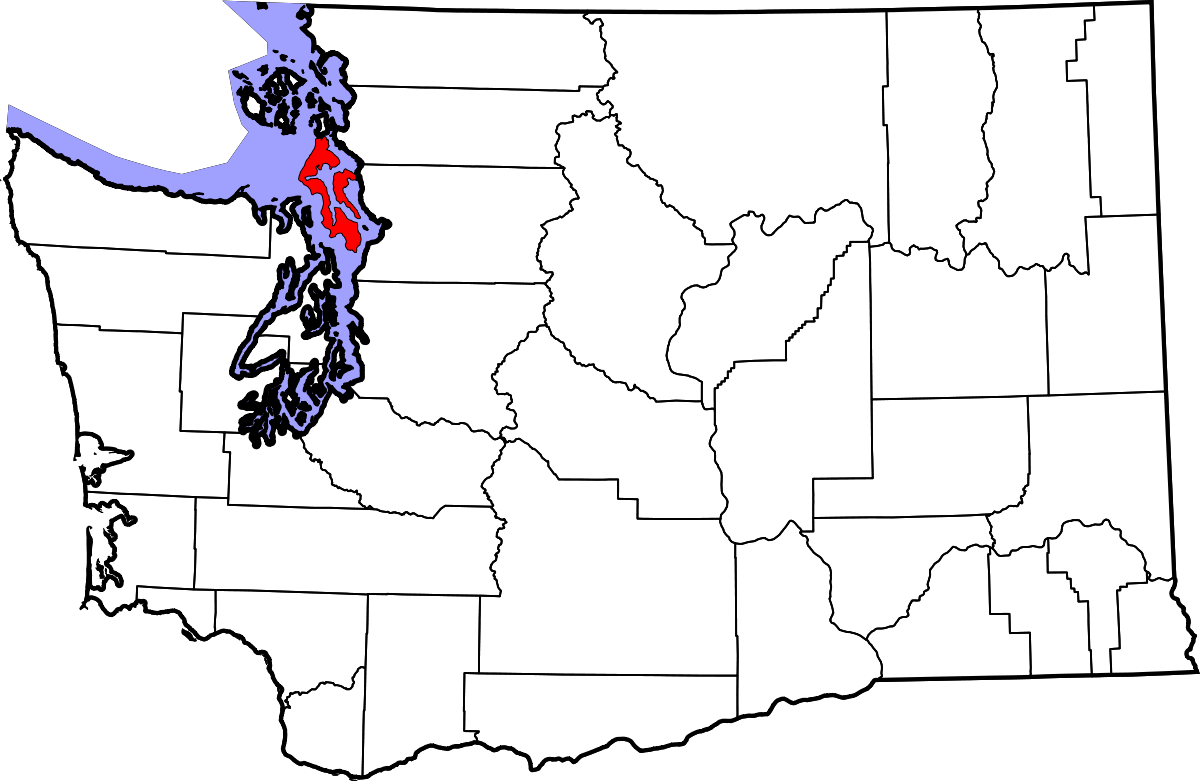
\includegraphics[width=0.75\textwidth]{imgs/islandcounty.png}
    \vfill
    \begin{minipage}{0.49\textwidth}
      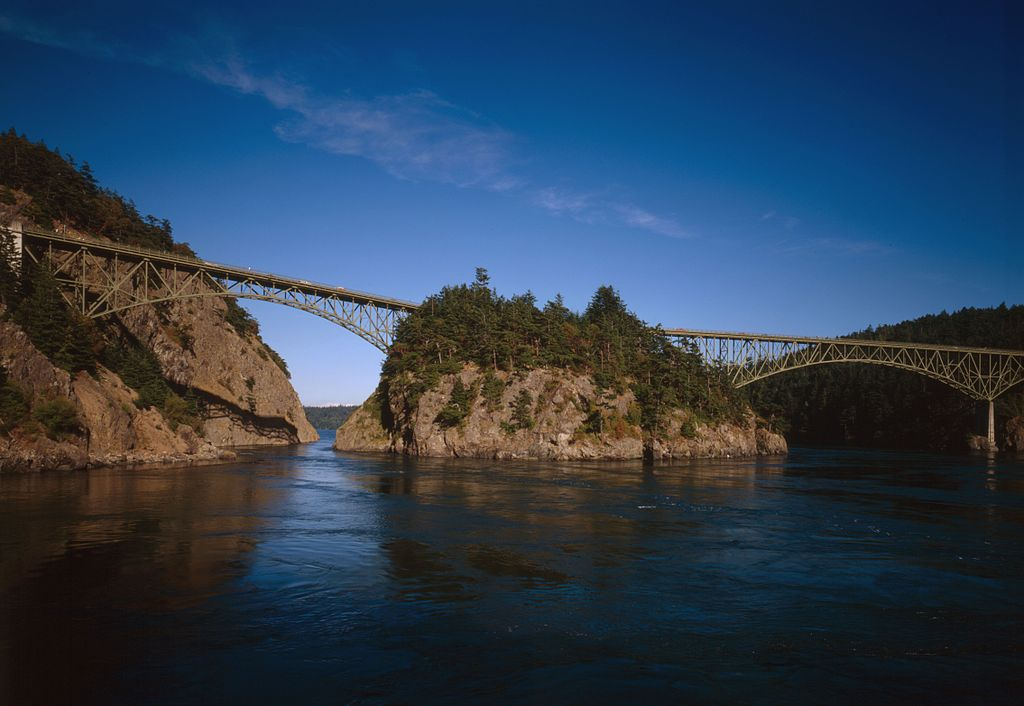
\includegraphics[width=\textwidth, height=75px]{imgs/roundeddeception.jpg}
    \end{minipage}
    \begin{minipage}{0.49\textwidth}
      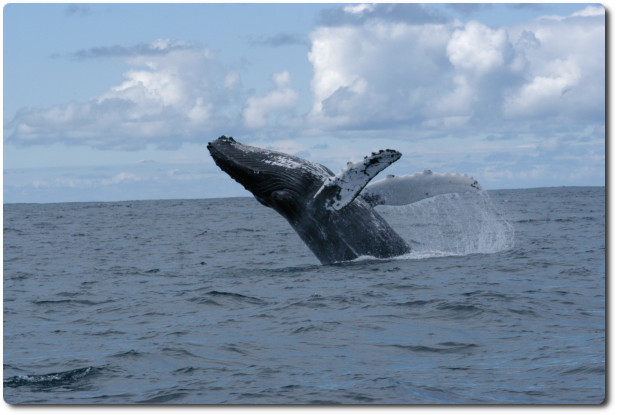
\includegraphics[width=\textwidth]{imgs/roundedgreywhale.pdf}
    \end{minipage}
  \end{minipage}
\end{frame}
\section{Java Basics}

\begin{frame}[fragile]
    \frametitle{\lstinline|static| in the main method}
    \begin{lstlisting}[frame=trBL]
class Foo{

    public static void main(String [] argv){
        System.out.println("Hello, world!");
    }

}
    \end{lstlisting}
    \vfill
    \begin{itemize}
        \item Why is this static!?
            \pause
        \item \textbf{Definition: } \lstinline|static| allows for a method or attribute to be used without needing to first instantiate a class
            \begin{itemize}
                \item We don't have to create an instance of \lstinline|Foo a = new Foo();| in order to call main.
            \end{itemize}
            \pause
        \item The \lstinline|main| method is the starting point for your program and the Java compiler needs to call it before instantiating any methods.
    \end{itemize}
\end{frame}

\begin{frame}[fragile]
    \frametitle{\lstinline|static| in the main method}
Off to the worksheet to compare the following classes!\\
\vfill
    \begin{minipage}{0.52\textwidth}
        \begin{lstlisting}[basicstyle=\tiny, frame=trBL]
class ComputeSumWithStatic{

  public static int sumNums(Integer[] nums){
    int total = 0;
    for(Integer num: nums){
      total += num;
    }
    return total;
  }
}

Integer[] n = {1, 2, 3, 4, 5};
int s = ComputeSumWithStatic.sumNums(n);
System.out.println(s);
        \end{lstlisting}
    \end{minipage}
    \hfill
    \begin{minipage}{0.45\textwidth}
        \begin{lstlisting}[basicstyle=\tiny, frame=trBL]
class ComputeSumWithoutStatic{

  public int sumNums(Integer[] nums){
    int total = 0;
    for(Integer num: nums){
      total += num;
    }
    return total;
  }
}

Integer[] n = {1, 2, 3, 4, 5};
ComputeSumWithoutStatic nonStaticSum = new ComputeSumWithoutStatic();
int s = nonStaticSum.sumNums(n);
System.out.println(s);
        \end{lstlisting}
    \end{minipage}
    \vfill
\end{frame}

\begin{frame}
    \frametitle{Access Modifiers}
    \begin{itemize}
        \item The follow
        \begin{itemize}
            \item \lstinline|public|: The attribute and method is accessible to any other class that instantiates, implements, or extends the class in which it resides.
            \item \lstinline|private|: The method or attribute is only accessible within the class.
            \item \lstinline|protected| and the default permissions serve other purposes.
        \end{itemize}
        \item For this class we primarily care about \lstinline|public| and \lstinline|private|.
    \end{itemize}
    
\end{frame}

\begin{frame}[fragile]
    \frametitle{Access Modifiers}
    \begin{minipage}{0.59\textwidth}
        \begin{lstlisting}[basicstyle=\tiny, frame=trBL]
class AnInt{
    
  public int num = 5;

  //..

}

AnInt x = new AnInt();
System.out.println(x.num); // You can read from it
x.num = 3;                 // You can write to it
        \end{lstlisting}
    \end{minipage}
    \begin{minipage}{0.39\textwidth}
        \scriptsize
        \begin{itemize}
            \item By declaring the attribute as public we can access them by using the format:
        \end{itemize}
        \begin{center}
            \lstinline|<instanceVar>.<attr>|
        \end{center}
    \end{minipage}
    \vfill
    \noindent\rule{\textwidth}{0.4pt}
    \vfill
    \begin{minipage}{0.59\textwidth}
        \begin{lstlisting}[basicstyle=\tiny, frame=trBL]
class AnInt{
    
  private int num = 5;

  //..

}

AnInt x = new AnInt();
System.out.println(x.num); // "read" error
x.num = 3;                 // "write" error
        \end{lstlisting}
    \end{minipage}
    \begin{minipage}{0.39\textwidth}
        \scriptsize
        \begin{itemize}
            \item By declaring it as private we no longer have read/write access to the attribute.
            \item How do we fix this?
            \begin{itemize}
                \item \scriptsize{getters and setters}
            \end{itemize}
        \end{itemize}
    \end{minipage}
\end{frame}

\begin{frame}[fragile]
    \frametitle{Getters and Setters}
    \begin{minipage}{0.59\textwidth}
        \begin{lstlisting}[basicstyle=\scriptsize, frame=trBL]
class AnInt{
    
  private int num = 5;
    
  public void setNum(int newNum){
    num = newNum;
  }

  public int getNum(){
    return num;
  }

}

AnInt x = new AnInt();
System.out.println(x.getNum()); 
x.setNum(3);
        \end{lstlisting}
    \end{minipage}
    \begin{minipage}{0.39\textwidth}
        \begin{itemize}
            \item Setters are used to change the values of private variables.
                \begin{itemize}
                    \item Good practice dictates we use the form \lstinline|set<VarName>|.
                \end{itemize}
                \pause
            \item Getters are used to retrieve the values of private variables.
                \begin{itemize}
                    \item Good practice dictates we use the form \lstinline|get<VarName>|.
                \end{itemize}
        \end{itemize}
    \end{minipage}
\end{frame}

\begin{frame}[fragile]
    \frametitle{Why use Getters and Setters?}
    \begin{minipage}{0.49\textwidth}
        \begin{lstlisting}[basicstyle=\tiny, frame=trBL]
class AnInt{
    
  private int num = 5;
    
  public void setNum(int newNum){
    num = newNum;
  }

  public int getNum(){
    return num;
  }

}

AnInt x = new AnInt();
System.out.println(x.getNum()); 
x.setNum(3);
        \end{lstlisting}
    \end{minipage}
    \begin{minipage}{0.49\textwidth}
        \begin{itemize}
            \item Why not leave everything public? That seems simpler!
            \item \textbf{Encapsulation} we want to hide as much of the internal representation of a class as possible.
        \end{itemize}
    \end{minipage}
\end{frame}

\begin{frame}[fragile]
    \frametitle{Why use Getters and Setters?}
    \begin{minipage}{0.49\textwidth}
        \begin{lstlisting}[basicstyle=\tiny, frame=trBL]
class APosInt{
    
  private int num = 1;
    
  public boolean setNum(int newNum){
    if(newNum > 0){
        num = newNum;
        return true;
    } else{
        return false;
    }   
  }

  public int getNum(){
    return num;
  }

}

APosInt x = new APosInt();
System.out.println(x.getNum()); 
x.setNum(3);
        \end{lstlisting}
    \end{minipage}
    \begin{minipage}{0.49\textwidth}
        \begin{itemize}
            \item Private variables and getters/setters allows us to control access to attributes via methods. For example:
            \begin{itemize}
                \item We can add checks to our setters to ensure what the user is setting is valid.
            \end{itemize}
        \end{itemize}
    \end{minipage}
\end{frame}

\begin{frame}[fragile]
    \frametitle{Why use Getters and Setters?}
    \begin{minipage}{0.49\textwidth}
        \begin{lstlisting}[basicstyle=\tiny, frame=trBL]
class AReadOnlyInt{
    
  private int num = 1;
    
  public int getNum(){
    return num;
  }

}

AReadOnlyInt x = new AReadOnlyInt();
System.out.println(x.getNum()); 
        \end{lstlisting}
    \end{minipage}
    \begin{minipage}{0.49\textwidth}
        \begin{itemize}
            \item Private variables and getters/setters allows us to control access to attributes via methods. For example:
            \begin{itemize}
                \item We can add checks to our setters to ensure what the user is setting is valid.
                \item We could only include a getter so that the user doesn't have write access to an attribute. 
            \end{itemize}
        \end{itemize}
    \end{minipage}
\end{frame}

\begin{frame}[fragile]
    \frametitle{Constructors}
    \begin{minipage}{0.49\textwidth}
        \begin{lstlisting}[basicstyle=\tiny, frame=trBL]
class AnInt{
    
  public int num; //define
  
  // Constructor # 1
  AnInt(){
    num = 0;
  }

  // Constructor # 2
  AnInt(int num){
    this.num = num;
  }

}

AnInt x = new AnInt(); 
AnInt y = new AnInt(2); 
        \end{lstlisting}
    \end{minipage}
    \begin{minipage}{0.49\textwidth}
        \begin{itemize}
            \item Constructors are used to: 1) initialize attributes and 2) perform any other setup instructions for a class.
                \pause
            \item If you don't define a constructor Java will provide a default one for you.
                \pause
            \item You can define multiple constructors with method overloading.
        \end{itemize}
    \end{minipage}
\end{frame}

\begin{frame}[fragile]
    \frametitle{toString Overrides}
    \begin{minipage}{0.49\textwidth}
        \begin{lstlisting}[basicstyle=\tiny, frame=trBL]
class AnInt{
    
  private int num;

  //..

  @Override
  public String toString(){
    return String.format("Our number is %d", num);
  }

}

AnInt x = new AnInt();
System.out.println(x); 
        \end{lstlisting}
    \end{minipage}
    \begin{minipage}{0.49\textwidth}
        \begin{itemize}
            \item The default toString produces a string of the format \lstinline|ClassName@memory-address|.
                \pause
            \item If we want to convert our class to a string or print it we want to override the \lstinline|toString| method.
                \pause
            \item String formatting is often the easiest way to accomplish this task:
                \begin{itemize}
                    \item \%d - A placeholder for ints
                    \item \%s - A placeholder for strings
                    \item \%f - A placeholder for floats
                \end{itemize}
        \end{itemize}
    \end{minipage}
\end{frame}

\begin{frame}
    \frametitle{Worksheet: Objects}
    \vfill
    In breakout rooms, work through the inclass activities for objects. We'll cover them once you get back.
    \vfill
\end{frame}


\section{ADTs and Interfaces}

\begin{frame}
    \frametitle{Abstract Data Types}
    \begin{itemize}
        \item ADTs are abstract! 
        \item They define behaviour but they do not define how that behaviour should be implemented.
        \begin{itemize}
            \item In Java this means that we usually implement them with interfaces. 
                \pause
            \item These define the methods, their parameters, and what they return.
                \pause
            \item A data structure then \lstinline|implements| the interface and \textit{must} implement each function in the interface.
                \pause
            \item Interfaces will be covered more in depth in future lectures.
        \end{itemize}
    \end{itemize}
\end{frame}

\begin{frame}[fragile]
    \frametitle{The List ADT}
    By implementing an interface we are required to provide an implemention for each method specified by the interface in order for our code to compile.
    \vfill
    \begin{minipage}{0.49\textwidth}
        \begin{lstlisting}[basicstyle=\tiny]
interface List{
    public void add(Object o);
    public void remove(int index);
    public Object get(int index);
    //...
}
        \end{lstlisting}
    \end{minipage}
    \begin{minipage}{0.49\textwidth}
        \begin{lstlisting}[basicstyle=\tiny]
class ArrayList implements List{
    public void add(Object o){
        //implementation here
    }
    //...
}

class LinkedList implements List{
    public void add(Object o){
        //a different implementation here
    }
    //...
}

List<Integer> A = new ArrayList<>();
List<Integer> B = new LinkedList<>();
        \end{lstlisting}
    \end{minipage}
\end{frame}


%\begin{frame}
%    \frametitle{Abstract Data Types}
%    %\textbf{The Listov Substitution Principle}
%    %\begin{quote}
%    %    Any subclass object should be substitutable for the superclass object from which it is dervied.
%    %\end{quote}
%    \begin{figure}
%        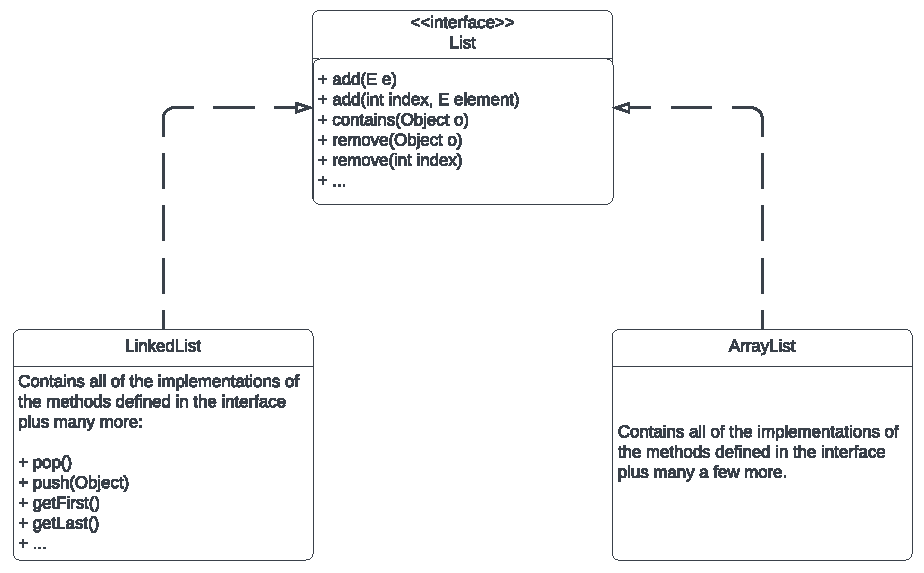
\includegraphics[width=200px]{imgs/list-adt.pdf}
%    \end{figure}
%\end{frame}

\section{List Implementations}

\begin{frame}[fragile]
    \frametitle{LinkedList}

    \begin{itemize}
        \item When we create a linked-list via \lstinline|List<Integer> numList = new LinkedList<>()| we have access to \textbf{\textit{only}} the \lstinline|List| interface's methods.
        \item When we create a linked-list via \lstinline|LinkedList<Integer> numList = new LinkedList<>()| we have access to these methods
        \begin{itemize}
            \item \lstinline|pop()| - Removes an element from the top of the list.
            \item \lstinline|push(Object o)| - Adds an element to the top of the list.
            \item \lstinline|getFirst()| - Returns the first element in the list.
            \item \lstinline|getLast()| - Returns the last element in the list.
            \item \lstinline|removeFirst()|- Removes \textbf{and returns} the first element in the list.
            \item \lstinline|removeLast()| - Removes \textbf{and returns} the last element in the list.
        \end{itemize}
    \end{itemize}
\end{frame}

\begin{frame}[fragile]
    \frametitle{ArrayList}
    \begin{itemize}
        \item When we create an arraylist via \lstinline|List<Integer> numList = new ArrayList<>()| we have access to \textit{\textbf{only}} the \lstinline|List| interface's methods.
        \item When we create an arraylist via \lstinline|ArrayList<Integer> numList = new ArrayList<>()| we have access to some additional methods.
    \end{itemize}
\end{frame}


\section{The List Interface}
\begin{frame}[fragile]
    \frametitle{Programming to Interfaces}
    \begin{minipage}{0.49\textwidth}
    Consider the following segment of code:
    \vfill
        \begin{lstlisting}[basicstyle=\tiny, frame=trBL]
public int sumList(List<Integer> lst){

  int total = 0;

  for(int i = 0; i < lst.size(); i++){
    total += lst.get(i);
  }

  return total;
}

List<Integer> a = new ArrayList<>();
List<Integer> b = new LinkedList<>();

// Fill them with numbers 1-10
for(int i = 1; i <= 10; i++){
  a.add(i);
  b.add(i);
}

System.out.println(sumList(a));
System.out.println(sumList(b));
        \end{lstlisting}
    \end{minipage}
    \begin{minipage}{0.49\textwidth}
        \begin{itemize}
            \item The two key takeaways from this segment of code:
                \begin{enumerate}
                    \scriptsize
                    \item We declared these as \lstinline|List| type rather than \lstinline|ArrayList| or \lstinline|LinkedList|. 
                        \begin{itemize}
                            \tiny
                            \item This limits the methods we can use on a and b to \textbf{only} those specified by the List interface.
                        \end{itemize}
                    \item The \lstinline|sumList| method takes a \lstinline|List| as a parameter.
                \end{enumerate}
        \end{itemize}
    \end{minipage}
\end{frame}

\begin{frame}[fragile]
    \frametitle{Programming to Interfaces}
    \begin{minipage}{0.49\textwidth}
    Consider the following segment of code:
    \vfill
        \begin{lstlisting}[basicstyle=\tiny, frame=trBL]
public float sumList(List<Integer> lst){

  int total = 0;

  for(int i = 0; i < lst.size(); i++){
    total += lst.get(i);
  }

  return total;
}

List<Integer> a = new ArrayList<>();
List<Integer> b = new LinkedList<>();

// Fill them with numbers 1-10
for(int i = 1; i <= 10; i++){
  a.add(i);
  b.add(i);
}

System.out.println(sumList(a));
System.out.println(sumList(b));
        \end{lstlisting}
    \end{minipage}
    \begin{minipage}{0.49\textwidth}
        \begin{itemize}
            \item \textbf{Key Takeaway \#1}: Methods should take \lstinline|List| as the parameter unless your method specifically requires methods only avaliable in the \lstinline|LinkedList| or \lstinline|ArrayList| classes.
            \item \textbf{Key Takeaway \#2}: Lists should be delcared as \lstinline|List| unless you require methods only avaliable in the \lstinline|LinkedList| or \lstinline|ArrayList| classes.
        \end{itemize}
    \end{minipage}
\end{frame}

\begin{frame}
    \frametitle{Worksheet: List ADT}
    \vfill
    In breakout rooms, work through the inclass activities for List ADT.  We'll cover them once you get back.
    \vfill
\end{frame}


\begin{frame}[fragile]
    \frametitle{Algorithm: Filtering a List}
    \begin{algorithm}[H]
        \caption{Filtering a List}
        \begin{algorithmic}[1]
            \Procedure{FilterList}{GivenList}
            \State NewList $\gets$ new List()
            \For{item $\in$ GivenList}
            \If{item meets criteria}
            \State NewList.add(item)
            \EndIf
            \EndFor
            \State \Return{NewList}
            \EndProcedure
        \end{algorithmic}
    \end{algorithm}
\end{frame}

\begin{frame}[fragile]
    \frametitle{Another Example of Programming to Interfaces}
    \centering
    \begin{lstlisting}[basicstyle=\scriptsize, frame=trBL]
public List<Integer> filterPosNums(List<Integer> lst){

    List<Integer> posLst = new ArrayList<>();

    for(int i = 0; i < lst.size(); i++){
        Integer item = lst.get(i);
        if(item > 0){
            posLst.add(item);
        }
    }

    return posLst;
}

    \end{lstlisting}
    \begin{itemize}
        \item Allows us to filter the positive integers from any \lstinline|List|.
        \item This algorithm doesn't require any methods specific to \lstinline|ArrayList| or \lstinline|LinkedList|.
    \end{itemize}
\end{frame}

\begin{frame}
    \frametitle{Worksheet: Filtering Lists}
    \vfill
    In breakout rooms, work through the inclass activities for filtering lists for ~15 minutes. We'll cover them once you get back.
    \vfill
\end{frame}

\section{The Integer Class}

\begin{frame}[fragile]
    \frametitle{Integer vs int}
    \begin{itemize}
        \item \lstinline|int| is a primative data type meaning it \textit{only} has the integer value stored.
            \pause
        \item \lstinline|Integer| is a wrapper class that contains the value and methods for working with integers.
            \pause
        \item \lstinline|Integer| has useful \lstinline|static| fields:
        \begin{itemize}
            \item \lstinline|MAX_VALUE| - The largest value an int can be.
            \item \lstinline|MIN_VALUE| - The minimum value an int can be.
        \end{itemize}
            \pause
        \item \lstinline|Integer| has useful \lstinline|static| methods:
        \begin{itemize}
            \item \lstinline|Integer.parseInt(String str)| - Attempts to convert a string representation of an integer (e.g., ``123'')  to an integer.
        \end{itemize}
            \pause
        \item and even some useful non-static methods. If we declare an integer as \lstinline|Integer integerInstance = new Integer(3)|:
        \begin{itemize}
            \item \lstinline|integerInstance.intValue()| - Returns the value of the integer as a primative int (i.e., 3).
            \item \lstinline|integerInstance.toString()| - Returns the value of the integer as a string (i.e., ``3'').
        \end{itemize}
    \end{itemize}
\end{frame}

\begin{frame}[fragile]
\frametitle{Integer to String Conversation and Exceptions}
    \begin{lstlisting}[basicstyle=\scriptsize, frame=trBL]
String str = // something...
try{
    Integer convInt = Integer.parseInt(str);
} catch(NumberFormatException e){
    System.out.printf("%s cannot be converted to an Integer", str);
}
    \end{lstlisting}
    \begin{itemize}
        \item We use the \lstinline|Integer.parseInt(str)| method to convert a given string (\lstinline|str|) to an \lstinline|Integer|.
        \begin{itemize}
            \item If \lstinline|str = "123"| this works fine!
            \item If \lstinline|str = "123asdf"| this produces a \lstinline|NumberFormatException| :-(
        \end{itemize}
        \pause
        \item An exception is an error (you've likely seen these). 
            \pause
        \item We use a try-catch block to manage exception
        \begin{itemize}
            \item We ``try'' the code in the try block
            \item If a specified exception occurs while trying the code we ``catch'' that exception and run the code in the catch block
        \end{itemize}
    \end{itemize}
\end{frame}

\begin{frame}[fragile]
    \begin{itemize}
        \item Week 1 practice has been released
        \item Implementation #1 - has been released
        \begin{itemize}
            \item Begin working on the Vehicle.java file.
        \end{itemize}
        \item Complete whenisgood. Office hours begin Thursday.
    \end{itemize}
\end{frame}

\end{document}
